\documentclass[12pt]{article}

\usepackage[margin=1.0in]{geometry}
\usepackage{graphicx}
\graphicspath{ {./} }

\begin{document}

\title{CS4347 : Database Systems\\Homework Assignment 2}
\author{Matthew McMillian\\mgm160130@utdallas.edu}
\maketitle



\begin{enumerate}
	
	\item Make a ER diagram following the st of requirements for a UNIVERSITY database that is used to keep track of students' transcripts. This is similar but not identical to the database shown in figure 1.2 in the textbook. \\
		\begin{center}
			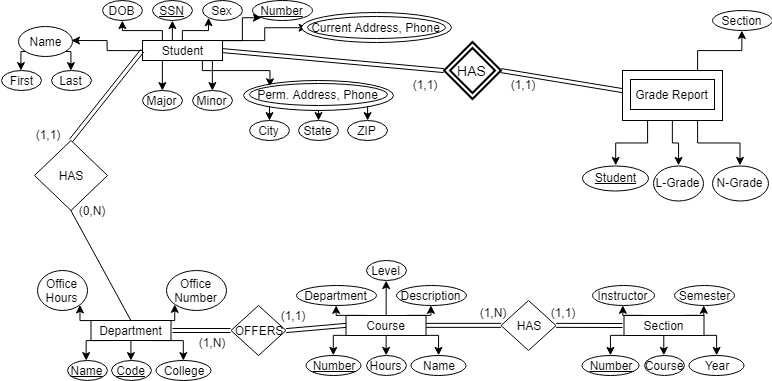
\includegraphics[scale=0.55]{er2}
		\end{center} 
		\pagebreak
	\item Design a complex attribute to hold data pertaining to a STUDENT entity type's previous college education. \\
	\begin{center}
			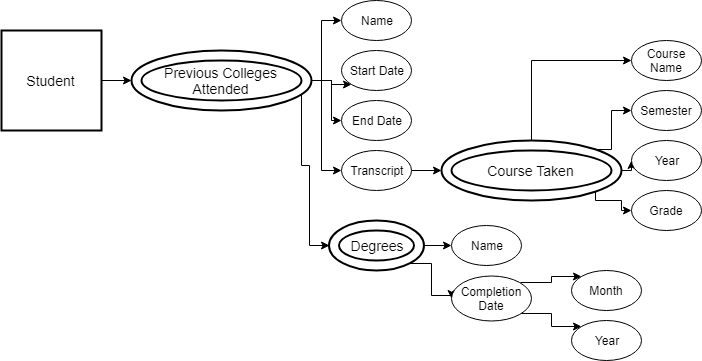
\includegraphics[scale=0.55]{attr}
		\end{center} 
	
\end{enumerate}


\end{document}
